\documentclass{beamer}
\setbeamercovered{transparent}
\usepackage{epstopdf}
\usepackage{listings}
\usepackage{lipsum}
\usepackage{subfig}
\usepackage{algorithm}
\usepackage{algorithmicx}
\usepackage{cite}
\usepackage{lipsum}
\usepackage{amssymb}
\usepackage{color}
\usepackage{IEEEtrantools}
\usepackage{booktabs}
\usepackage{texpower}
\usepackage{amsmath}
\usepackage{caption}
\usepackage{multirow}
\usepackage{graphicx}
\newtheorem{Key points}{Key points}
\newtheorem{Summary}{Summary}
\usepackage{dblfloatfix}
%\usepackage{adjustbox}
%\usepackage{animate}
%\usepackage{movie15}
%\usepackage{subfig}
%\newtheorem{Definition}{Definition}
%\usepackage[font={small}]{caption}
\usepackage{beamerthemeshadow}
\newcommand\Fontvi{\fontsize{5}{6.2}\selectfont}
\newcommand\Fontvia{\fontsize{6}{7.2}\selectfont}
\newcommand\Fontviaa{\fontsize{8}{7.2}\selectfont}
\usepackage{listings}
\lstset{language=C++,
                keywordstyle=\color{blue},
                stringstyle=\color{red},
                commentstyle=\color{green},
                morecomment=[l][\color{magenta}]{\#},
                numbers=left,
                escapeinside=||
}

%\captionsetup{font=scriptsize,labelfont=scriptsize}
 \usetheme{Berkeley}%PaloAlto 
\begin{document}
\title[Linear Algebra Introduction]{Data Science prerequisite} 
\author{Ahsan Ijaz}
\date{}
 \frame{\titlepage}
% \AtBeginSection[]
% {
% \begin{frame}<beamer>{Table of Contents}
% \tableofcontents[currentsection,currentsubsection, 
%     hideothersubsections, 
%     sectionstyle=show/shaded,
% ]
% \end{frame}
% }
\section{Linear Algebra}
\subsection{Spaces}
 \begin{frame}
   \frametitle{Linear Algebra}
   The very basic:
  Adding two Vectors.

   \begin{equation*}
     c\mathbf{v} +d\mathbf{w} = c\begin{bmatrix}
1\\ 
1\\ 
\end{bmatrix}+
d\begin{bmatrix}
2\\
3\\
\end{bmatrix}
   \end{equation*}
   \begin{definition}
     The sum of \emph{cv} and \emph{dw} is a linear combination of \emph{v} and \emph{w}.
   \end{definition}
   \begin{itemize}
   \item<2-> How would \emph{cv} look like in space?
   \item<3-> How would \emph{cv + dw} look like in space?
   \end{itemize}

\uncover<4>{We will come back to this later...}
 \end{frame}

 \begin{frame}
   \frametitle{Dot Product}
 \begin{itemize}
 \item Length of a vector. $\lVert{}v{}\rVert = \mathbf{v.v}$
\item Unit vector : $\frac{v}{\lVert{}v{}\rVert}$
\item Dot Product zero when vectors are perpendicular.
 \end{itemize}
   \begin{equation*}
     \mathbf{v.w}=v_1w_1+v_2w_2
   \end{equation*}
 \end{frame}

 \begin{frame}
   \frametitle{Matrices}
   \begin{equation*}
     u=\begin{bmatrix}
      1\\-1\\0
     \end{bmatrix}\qquad{}v=
     \begin{bmatrix}
       0\\1\\-1
     \end{bmatrix}\qquad{}w=
     \begin{bmatrix}
       0\\0\\1
     \end{bmatrix}
   \end{equation*}
\uncover<2->\textbf{Linear Combination:}
\begin{equation*}
  c\begin{bmatrix}
      1\\-1\\0
     \end{bmatrix}+d
\begin{bmatrix}
       0\\1\\-1
     \end{bmatrix}
+e\begin{bmatrix}
       0\\0\\1
     \end{bmatrix}=
      \begin{bmatrix}
        c\\d-c\\e-d
      \end{bmatrix}
\end{equation*}
\uncover<3->\textbf{We can re-write it as:}
\begin{equation*}
  \begin{bmatrix}
      1 & 0& 0\\
      -1 & 1 & 0\\
       0 & -1 & 1
     \end{bmatrix}
 \begin{bmatrix}
       c\\d\\e
     \end{bmatrix}=
       \begin{bmatrix}
        c\\d-c\\e-d
      \end{bmatrix}
    \end{equation*}
 \end{frame}
 \begin{frame}
   \frametitle{Matrices}
   \textbf{We can re-write it as:}
\begin{equation*}
  \begin{bmatrix}
      1 & 0& 0\\
      -1 & 1 & 0\\
       0 & -1 & 1
     \end{bmatrix}
 \begin{bmatrix}
       c\\d\\e
     \end{bmatrix}=
       \begin{bmatrix}
        c\\d-c\\e-d
      \end{bmatrix}
    \end{equation*}

   \textbf{Alternatively:}
    \begin{equation*}
      \mathbf{A}x=
      \begin{bmatrix}
        u & v & w
      \end{bmatrix}
      \begin{bmatrix}
        c\\d\\e
      \end{bmatrix}=
        \mathbf{b}
    \end{equation*}
Here, consider $x$ as input, $A$ as the system model and $b$ as the output.
 \end{frame}
 \begin{frame}
   \frametitle{Digression-Matrices: Dot Product picture}
  \begin{equation*}
     Ax=   \begin{bmatrix}
      1 & 0& 0\\
      -1 & 1 & 0\\
       0 & -1 & 1
     \end{bmatrix}
     \begin{bmatrix}
       x_1\\x_2\\x_3
     \end{bmatrix}
=
\begin{bmatrix}
  (1,0,0).(x_1,x_2,x_3)\\
(-1,1,0).(x_1,x_2,x_3)\\
(1,-1,1).(x_1,x_2,x_3)
\end{bmatrix}
   \end{equation*}
 \end{frame}
 \begin{frame}
   \frametitle{Ax=b}
   \textbf{Think of $b$ as known and look for $x$ that solves it.}
   \begin{itemize}
   \item \emph{Old Question:} Compute linear combination of $x_1u + x_2v + x_3w$ to find $b$.
\item \emph{New Question:} Which combination of $u,v,w$ produce a particular vector $b$.
   \end{itemize}
 \end{frame}
\subsection{Definitions}
 \begin{frame}
   \frametitle{Independence and Dependence}
   \begin{itemize}
   \item Matrix has no inverse.
   \item One of the vectors is the linear combination of other vectors.
   \end{itemize}
 \end{frame}
 \begin{frame}
   \frametitle{Column Space}
   In $\mathbf{Ax}=\mathbf{b}$, what happens if we take all linear combinations of the columns of $\mathbf{A}$?
\begin{itemize}
   \item Equivalent of multiplying $A$ with every possible $x$.
   \end{itemize}
 \uncover<2->{\begin{definition}
     The \textbf{column space} consists of all \textbf{linear combinations of the columns.} The combinations are all possible vectors $Ax$.
   \end{definition}}
 \begin{itemize}
 \item<3-> To solve $Ax=b$ is to express b as the linear combination of the columns of A.
\item<4-> The system $Ax=b$ is solvable only if $b$ is in the column space of $A$~($C(A)$).
 \end{itemize}
 \end{frame}
 \begin{frame}
   \frametitle{Dimension, Basis}
   \begin{definition}
    Dimension is the space that the columns of $A$ can span.
   \end{definition}
\uncover<2->{   \begin{definition}
     Basis is the first $n$ vectors of the matrix $A$ that span the whole space.
   \end{definition}}
 \begin{itemize}
 \item<3-> The columns of $A$ are \textbf{independent} if $x=0$ is the only solution of $Ax=0$.
\item<4-> The vectors $v_1,v_2,\cdots,v_n$ span the space if their combinations fill the space.
\item<5-> Any $n$ independent vectors in $R^n$ must span $R^n$ so they are basis. 
 \end{itemize}
 \end{frame}
\subsection{Projections}
 \begin{frame}
   \frametitle{Projections}
   \begin{itemize}
   \item What are the projections of $b=(2,3,4)$ onto the z-axis and the xy plane?
   \item<2-> What matrices produce those projections onto a line and a plane?
   \end{itemize}
\uncover<3->{ The projection matrix \textbf{P} multiplies \textbf{b} to give \textbf{p}.
  Onto the z-axis:
   \begin{equation*}
     P_1=\begin{bmatrix}
       0 & 0 & 0\\
       0 & 0 & 0\\
       0 & 0 & 1
     \end{bmatrix}
   \end{equation*}
}

\uncover<4->{Onto the xy plane:
   \begin{equation*}
     P_1=\begin{bmatrix}
       1 & 0 & 0\\
       0 & 1 & 0\\
       0 & 0 & 0
     \end{bmatrix}
   \end{equation*}
}
 \end{frame}
 \begin{frame}
   \frametitle{Continuation: Projection}
   \begin{figure}
\centering
\subfloat{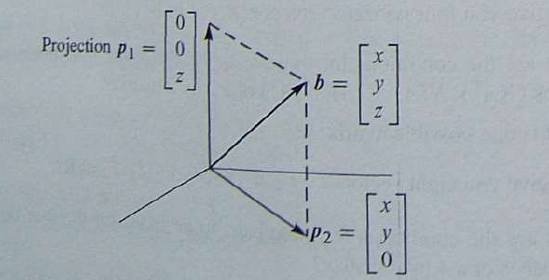
\includegraphics[width=0.7\columnwidth]{proj}} 
\caption{Projection $\mathbf{p_1=P_1b}$ and $\mathbf{p_2=P_2b}$ onto the z-axis and xy-plane}
\end{figure}
What does $p_1 + p_2$ gives???
 \end{frame}
 \begin{frame}
   \frametitle{Projection onto subspaces}
   \begin{itemize}
   \item    Projecting the given vector onto the column space of A. 
\item<2-> Problem is to project any $b$ onto the column space of any $m by n$ matrix.
   \end{itemize}
 \end{frame}

 \begin{frame}
   \frametitle{Projection Onto a Line}
   \textbf{{\color{red}Problem Statement:}} Find the point $p$  closest to $b$ on a line in the direction of $a$.
\begin{columns}[onlytextwidth]
    \begin{column}{0.4\textwidth}
      \centering
   \begin{itemize}
   \item Let $p=\hat{x}a$.
   \item<2-> error $e=b-\hat{x}a$
   \item<3-> $a.(b-\hat{x}a)=0$
   \item<4-> or $a.b - \hat{x}a.a=0$
   \item<5-> $\hat{x}=\frac{a.b}{a.a}=\frac{a^Tb}{a^Ta}$
   \end{itemize}
\end{column}
    \begin{column}{0.6\textwidth}
      \centering
\begin{figure}
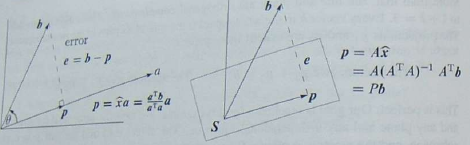
\includegraphics[width=1\columnwidth]{projline}\\
\end{figure}
    \end{column}
\end{columns}
 \end{frame}
 \begin{frame}
   \frametitle{Projection Example}
   Project $b=(1,1,1)$ onto $a=(1,2,2)$ to find $p=\hat{x}a$.
   \begin{itemize}
   \item<2-> $a^Tb=5$
   \item<3-> $a^ta=9$
   \item<4-> $p=\frac{5}{9}a$
   \item<5-> $e=b-p$
   \item<6-> $p=(\frac{5}{9},\frac{10}{9},\frac{10}{10})$ and $e=(\frac{4}{9},-\frac{1}{9},-\frac{1}{9})$
   \end{itemize}
\uncover<7->{What should be $e^Ta$ ??}
 \end{frame}

 \begin{frame}
   \frametitle{Alternate Projection}
   \begin{center}
     \begin{itemize}
     \item $\lVert{}p\rVert= \lVert{}b\rVert{}\cos\theta$
     \item $\lVert{}e\rVert=\lVert{}b\rVert{}\sin\theta$
     \end{itemize}
   \end{center}
\uncover<2-> {
  \begin{definition}
    Projection Matrix $\mathbf{P}$:
    \begin{equation*}
      p = a\hat{x} = a\frac{a^Tb}{a^Ta}=Pb
    \end{equation*}
\emph{where the matrix is} $\mathbf{P}=\frac{aa^T}{a^Ta}$
  \end{definition}
}
 \end{frame}
 \begin{frame}
   \frametitle{Projection: Example 2}
   Find Projection matrix onto the line through $a=(1,2,2)$.
   \begin{itemize}
   \item<2-> \begin{equation*}
p=\frac{aa^T}{a^Ta}=\frac{1}{9}
     \begin{bmatrix}
       1\\2\\2
     \end{bmatrix}[1~~2~~2]=
    \frac{1}{9} \begin{bmatrix}
       1 & 2 & 2\\
       2 & 4 & 4\\
       2 & 4 & 4
     \end{bmatrix}
        \end{equation*}
\item<3-> This matrix projects any vector $b$ onto $a$.
\item<4->
  \begin{equation*}
        \frac{1}{9} \begin{bmatrix}
       1 & 2 & 2\\
       2 & 4 & 4\\
       2 & 4 & 4
     \end{bmatrix}
     \begin{bmatrix}
       1\\1\\1
     \end{bmatrix}
=\frac{1}{9}
\begin{bmatrix}
  5\\10\\10
\end{bmatrix}
  \end{equation*}
   \end{itemize}
 \end{frame}

 \begin{frame}
   \frametitle{Projection properties}
   \begin{itemize}
   \item<2-> What would $\mathbf{P}^2$ give??
   \item<3-> What would be $P$ if we use $2a$??
   \item<4-> What would $(\mathbf{I}-\mathbf{P})b$ be?
   \end{itemize}
 \end{frame}
 \begin{frame}
   \frametitle{Projection Multi-dimension}
   \begin{itemize}
   \item<2-> $A^T(b-A\hat{x})=0$ or $A^TA\hat{x}=A^Tb$
\item<3-> $p=A\hat{x}=A(A^TA)^{-1}A^Tb$
\item<4-> $P=A(A^TA)^{-1}A^T$
   \end{itemize}
 \end{frame}
\subsection{Orthonormality}
 \begin{frame}
   \frametitle{Orthonormal Basis}

\begin{definition}
  The vectors are orthonormal if:
  \uncover<2->{\begin{center}
  \begin{equation*}
      q_i^Tq_j=
      \begin{cases}
        0, & when\qquad{}i\ne{}j\qquad{}\text{orthogonal vectors}\\
        1, & when\qquad{} i=j\qquad{} \text{orthonormal}
      \end{cases}
    \end{equation*}
  \end{center}}
 A matrix with orthonormal columns is assigned the letter $\mathbf{Q}$.
\end{definition}
\begin{itemize}
\item<3-> $\mathbf{Q^TQ=I}$
\item<4-> $Q^T=Q^{-1}$
\end{itemize}
\end{frame}
 \begin{frame}
   \frametitle{Projection using Orthonormal basis}
   \begin{itemize}
    \item Let $p=\hat{x}q$.
    \item<2-> error $e=b-\hat{x}q$
    \item<3-> $q.(b-\hat{x}q)=0$
    \item<4-> or $q.b - \hat{x}q.q=0$
    \item<5-> $\hat{x}=\frac{q.b}{q.q}=\frac{q^Tb}{q^Tq}$
    \item<6-> $\hat{x}=q^Tb$
    \item<7-> $q^Tb= \lvert{}b\rvert\cos\theta$
    \item<8-> $(q^Tb)q= \text{Projection of \emph{b} in the direction of \emph{q}}$
\item<9-> $P=Q(Q^TQ)^{-1}Q^T = QQ^T$
   \end{itemize} 
\end{frame}
\begin{frame}
  \frametitle{Projection using Orthonormal basis}
Projection onto $q's$
\uncover<1>{   \begin{definition}
     \begin{equation*}
       P=
       \begin{bmatrix}
         q_1 & \cdots & q_n
       \end{bmatrix}
       \begin{bmatrix}
         q_1^T\\.\\.\\.\\q_N^T
       \end{bmatrix}b=        \begin{bmatrix}
         q_1 & \cdots & q_n
       \end{bmatrix}
       \begin{bmatrix}
         q_1^Tb\\.\\.\\.\\q_N^Tb
       \end{bmatrix}
     \end{equation*}
   \end{definition}
}
\uncover<2->{So $b$ can be written as:
\begin{center}
\large{
  \begin{equation*}
    {\color{red}\mathbf{b=q_1(q_1^Tb)+q_2(q_2^Tb)+\cdots+q_n(q_n^Tb)}}
  \end{equation*}
}
\end{center}
}
\end{frame}
%\subsection{Conclusive Equation}
\begin{frame}
  \frametitle{Conclusive Equation: }
  \begin{center}
  \begin{equation*}
    {\color{red}\mathbf{b=q_1(q_1^Tb)+q_2(q_2^Tb)+\cdots+q_n(q_n^Tb)}}
  \end{equation*}
\large{The vector $b$ has been broken down into perpendicular pieces. Then, by adding the pieces, we can put back the vector again.}
\end{center}
\end{frame}
\section{Transforms}
\subsection{Dot Product of Functions}
\begin{frame}
  \frametitle{Transforms}
\large
{\color{blue}Breaking down:} Transform \\
   \begin{figure}
\centering
\subfloat{
\includegraphics[width=0.4\columnwidth]{humptyb}} 
\caption{Transform}
\end{figure}
 {\color{blue}Putting back together:} Inverse Transform (King's men didn't know how to.)
\end{frame}
\begin{frame}
  \frametitle{Dot Product Continuous space}
  The standard inner product for complex valued functions is:
  \begin{equation*}
    f.g= \int_{-\infty}^{\infty}{f(t)g^*(t)dt}    \end{equation*}
Compare it with vector space:
\begin{equation*}
    a.b= a^Tb = \sum_{i=0}^n{a_ib_i^*}   \footnotemark 
\end{equation*}
\footnotetext[1]{*: Remember Hermitian matrix? Transpose of complex matrix is taken by inverting signs of complex values and changing rows and columns afterwards.}
\end{frame}
\subsection{Fourier series}
\begin{frame}
  \frametitle{Fourier Series }
  Calculating coefficients: (breaking down:)
  \begin{eqnarray*}
  a_0 & = &  \frac{1}{\pi}\int_{2\pi}{f(x)dx}\\ 
  a_n & = &  \frac{1}{\pi}\int_{2\pi}{f(x)\cos{nx}dx}\\
  b_n & = &  \frac{1}{\pi}\int_{2\pi}{f(x)\sin{nx}dx} 
  \end{eqnarray*}
(putting back together:)
  \begin{equation*}
    f(x)= \frac{a_0}{2}+ \sum_{n=1}^{\infty}[a_n\cos{nx}+b_n\sin{nx}]
  \end{equation*}
\end{frame}
\begin{frame}
  \frametitle{Fourier Series}
\Fontviaa
  \begin{equation*}
     {\color{magenta}f(x)}= \sum_{n=0}^{\infty}\left[\left({\color{blue}\frac{1}{\pi}\int_{2\pi}{{\color{magenta}f(x)}\cos{nx}dx}}\right){\color{red}\cos{nx}}+\left({\color{blue}\frac{1}{\pi}\int_{2\pi}{{\color{magenta}f(x)}\sin{nx}dx}}\right){\color{red}{\color{red}\sin{nx}}}\right]
  \end{equation*}
  \begin{equation*}
    {\color{magenta}b}=({\color{blue}q_1^T{\color{magenta}b}}){\color{red}q_1}+({\color{blue}q_2^T{\color{magenta}b}}){\color{red}q_2}+\cdots+({\color{blue}q_n^T{\color{magenta}b}}){\color{red}q_n}
  \end{equation*}
\vfill
\uncover<2->{{\color{magenta} Function/Vector/Signal/Control Input,...}\\
{\color{red} Orthonormal Basis Function, Orthonormal Vectors,...}\\
Brackets (): Dot Product/Inner Product/Convolution~(special case),...\\
}
\end{frame}
\subsection{Comparative Discussion}
\begin{frame}
  \frametitle{Other Transforms}
Laplace Transform:
\uncover<2->  {\begin{equation*}
    F(s)= \int_0^\infty{f(t)e^{-st}dt}
  \end{equation*}
}
\uncover<3->
{Z-Transform:
\begin{equation*}
  X(z)=\sum_{n=-\infty}^{\infty}x[n]z^{-n}
\end{equation*}}
\uncover<4->{Power Series:
  \begin{equation*}
    f(x)= a_0 + a_1x + a_2x^2 + \cdots = \sum_{n=0}^{\infty}{a_nx^n}
  \end{equation*}
}
\uncover<5-> Taylor series, Wavelet transforms, Maclaurin Series ...
\end{frame}
\end{document}
%%% Local Variables:
%%% mode: latex
%%% TeX-master: t
%%% End:
